\chapter{Development And Implementation}
\section{The Linux Kernel}
The Linux kernel is a monolithic Unix-like computer operating system kernel. The Linux operating system is based on it and deployed on both traditional computer systems such as personal computers, servers and small system on chip computers; usually in the form of Linux distributions, and on various embedded devices such as routers, wireless access points, PBXes, set-top boxes, FTA receivers, smart TVs, PVRs and NAS appliances. The Android operating system for tablet computers, smartphones and smart-watches is also based atop the Linux kernel.\\
The Linux kernel was conceived and created in 1991 by Linux Torvalds for his personal computer and with no cross-platform intentions, but has since expanded to support to huge array of computer architecture, many more than other operating systems or kernels. Linux rapidly attracted developers and users who adopted it as the kernel for other free software projects, notably the GNU Operating System. The Linux kernel has received contributions from nearly 12,000 programmers from more than 1,200 companies, including some of the largest software and hardware vendors.
\subsection{The Linux Device Driver Model}
Linux today supports more hardware devices than any other operating system in the history of the world. It does this using a development model significantly different from the familiar Windows device driver model. The Linux development process continues to evolve to better support the needs of Independent Hardware Vendors (IHVs), distributions, and other members of the community, and the advantages of the Linux model are increasing with time. While Linux will not provide a stable source or binary interface for driver developers, IHVs should familiarize themselves with a number of useful projects, many sponsored by the Linux Foundation, that ease driver development, including the Hardware NDA program, the Linux Drivers Project, and the Driver Backport Workgroup. When IHVs engage with the Linux community, they almost invariably find that the Linux driver model provides significant benefits that lower their costs while producing better drivers.
\subsubsection{Overview}
A fundamental purpose for operating systems (OSes) is to serve as an abstraction layer between applications and hardware to enable interoperability. An IHV wants their hardware to be able to make use of all the relevant features of an OS, and an OS wants to take full advantage of the hardware it's running on. Since both the OS and the hardware tend to add and to rearrange features over time, it is a dynamic interaction. What everybody wants is for the hardware to “Just Work” without hassles or support calls.\\
Today, Linux works with more devices than any other OS in the history of the world.
\subsubsection{Driver Model}
The Linux driver model is different. For users, the goal is to provide the “Just Works” experience. The Linux model is that IHVs get the source code for their driver accepted into the mainline kernel. This entails a public peer review process to ensure that the driver code is of sufficient quality and does not have obvious bugs or security risks. Linux has neither a stable binary driver ABI nor a stable source-code driver Application Programming Interface (API). That is, there is no guarantee that an interface provided in one version of the kernel will be available in the next version, and portions of the ABI and API change in every kernel release.\\
By contrast, the Linux kernel does provide a stable user-space interface for Linux applications. These applications essentially have a contract with the Linux kernel that the user-space binary interfaces they rely on will continue to work consistently over time. That's why a pre-compiled Linux application can run correctly on multiple distributions and multiple versions. The underlying implementation of the user-space binary interfaces can and does change, but even an application compiled for pre-1.0 Linux will run correctly on the latest kernel. This is the opposite of device drivers, which have no guarantee whatsoever that any interface they rely on, whether binary or source, will remain consistent between versions of the kernel.\\
Counterintuitive though it might be from a proprietary viewpoint, this lack of internal kernel interface stability is preferable because both the kernel code and all of the drivers relying on it are open source. In fact, driver code is an integral part of the Linux operating system, not a second-class add-on. Once a driver is accepted into the mainline kernel, it will be maintained over time as internal kernel interfaces change. That is, when a subsystem maintainer accepts a patch to make an incompatible change to a kernel interface, that patch will simultaneously upgrade every driver that relies on the interface. And, new drivers and any upgrades to them automatically flow downstream from the mainline kernel to all Linux distributions.\\
The key strength of this approach from the user's viewpoint is that, in happy contrast with proprietary operating systems like Windows Vista, once a device is working on a given version of Linux, that support continues through all future versions. (Devices are generally only removed when they have become so rare that no users can be found.) In Linux, hardware support only gets better; it never gets worse.\\
From the IHV's point of view, the big benefit is that an IHV's driver is maintained over time by the community, meaning that other people fix, tune, and add features to the driver. When internal kernel interfaces change in each new OS release, IHVs don't need to write and release a new driver; their driver is upgraded automatically. Obsolete interfaces can be deprecated and removed rather than being maintained indefinitely. Common subsystems can be factored out of drivers, enabling leaner, less buggy device drivers while adding more functionality for all hardware. This improves the stability, security, and maturity of both the OS and the driver.\\
In addition, the Linux model enables cross-architecture driver support nearly for free. Even when an IHV only tests their driver on one chip architecture, interested developers ensure that the driver works with every architecture that Linux supports, which is more than any other OS in history. The strength of this approach has been especially apparent over the last decade as many chip architectures have moved from the 32 to 64 bits. Nearly all Linux drivers were quickly updated to support these newer architectures, while driver support for 64-bit Windows Vista even on the highest volume x86 architecture remains extremely poor today.\\
The biggest hurdle of the Linux driver model for some IHVs is the need to open source their driver code, which a small (but thankfully dwindling) number have been reluctant to do. Also, once a driver is accepted into the mainline, it can take up to 18 months to be deployed into an enterprise distro. It has not until now been convenient to backport the driver to existing distros, but that is improving with the Driver Backport Workgroup.\\
Having hardware reliably supported by Linux means getting the driver accepted into the mainline kernel. Supporting an out-of-mainline open source driver creates significant, never-ending support costs for the IHV, as new versions constantly need to be released as the kernel API changes. Supporting an out-of-mainline binary driver means even bigger, never-ending support costs for the IHV, and directly contradicts the recent statement by a large number of kernel developers that binary drivers are “undesirable”.\\
The Linux driver model is different from the Windows model many IHVs are used to. But it is a consistent and compelling approach, and has been successful at supporting nearly the entire universe of computer hardware. Moreover, the vast majority of all IHVs have adapted to Linux and have thriving businesses that work with the Linux driver development model.
\subsection{Overview of SPI support in Linux}
\subsubsection{What is SPI?}
The "Serial Peripheral Interface" (SPI) is a synchronous four wire serial link used to connect microcontrollers to sensors, memory, and peripherals. It's a simple "de facto" standard, not complicated enough to acquire a standardization body.  SPI uses a master/slave configuration.\\
The three signal wires hold a clock (SCK, often on the order of 10 MHz), and parallel data lines with "Master Out, Slave In" (MOSI) or "Master In, Slave Out" (MISO) signals.  (Other names are also used.)  There are four clocking modes through which data is exchanged; mode-0 and mode-3 are most commonly used.  Each clock cycle shifts data out and data in; the clock doesn't cycle except when there is a data bit to shift.  Not all data bits are used though; not every protocol uses those full duplex capabilities.\\
SPI masters use a fourth "chip select" line to activate a given SPI slave device, so those three signal wires may be connected to several chips in parallel.  All SPI slaves support chipselects; they are usually active low signals, labeled nCSx for slave 'x' (e.g. nCS0).  Some devices have other signals, often including an interrupt to the master. \\
Unlike serial busses like USB or SMBus, even low level protocols for SPI slave functions are usually not interoperable between vendors (except for commodities like SPI memory chips).
\begin{itemize}
	\item SPI may be used for request/response style device protocols, as with touchscreen sensors and memory chips.
	\item It may also be used to stream data in either direction (half duplex), or both of them at the same time (full duplex).
	\item Some devices may use eight bit words.  Others may use different word     lengths, such as streams of 12-bit or 20-bit digital samples.
	\item Words are usually sent with their most significant bit (MSB) first, but sometimes the least significant bit (LSB) goes first instead.
	\item Sometimes SPI is used to daisy-chain devices, like shift registers.
\end{itemize}
In the same way, SPI slaves will only rarely support any kind of automatic discovery/enumeration protocol.  The tree of slave devices accessible from a given SPI master will normally be set up manually, with configuration tables.\\
SPI is only one of the names used by such four-wire protocols, and most controllers have no problem handling "MicroWire" (think of it as half-duplex SPI, for request/response protocols), SSP ("Synchronous Serial Protocol"), PSP ("Programmable Serial Protocol"), and other related protocols.\\
Some chips eliminate a signal line by combining MOSI and MISO, and limiting themselves to half-duplex at the hardware level. In fact some SPI chips have this signal mode as a strapping option.  These can be accessed using the same programming interface as SPI, but of course they won't handle full duplex transfers.  You may find such chips described as using "three wire" signaling: SCK, data, nCSx. (That data line is sometimes called MOMI or SISO.) \\
Microcontrollers often support both master and slave sides of the SPI protocol.  This document (and Linux) currently only supports the master side of SPI interactions.
\subsubsection{Who uses SPI?}
Linux developers using SPI are probably writing device drivers for embedded systems boards.  SPI is used to control external chips, and it is also a protocol supported by every MMC or SD memory card.  (The older "DataFlash" cards, predating MMC cards but using the same connectors and card shape, support only SPI.)  Some PC hardware uses SPI flash for BIOS code. \\
SPI slave chips range from digital/analog converters used for analog sensors and codecs, to memory, to peripherals like USB controllers or Ethernet adapters; and more. \\
Most systems using SPI will integrate a few devices on a mainboard. Some provide SPI links on expansion connectors; in cases where no dedicated SPI controller exists, GPIO pins can be used to create a low speed "bitbanging" adapter.  Very few systems will "hotplug" an SPI controller; the reasons to use SPI focus on low cost and simple operation, and if dynamic reconfiguration is important, USB will often be a more appropriate low-pincount peripheral bus. \\
Many microcontrollers that can run Linux integrate one or more I/O interfaces with SPI modes. Given SPI support, they could use MMC or SD cards without needing a special purpose MMC, SD or SDIO controller.
\subsubsection{The SPI programming interface}
The linux/spi/spi.h header file includes kerneldoc, as does the main source code, and you should certainly read that chapter of the kernel API document.  This is just an overview, so you get the big picture before those details. \\
SPI requests always go into I/O queues.  Requests for a given SPI device are always executed in FIFO order, and complete asynchronously through completion callbacks.  There are also some simple synchronous wrappers for those calls, including ones for common transaction types like writing a command and then reading its response. \\
There are two types of SPI driver, here called: \\
Controller drivers ... controllers may be built into System-On-Chip 	processors, and often support both Master and Slave roles. 	These drivers touch hardware registers and may use DMA. 	Or they can be PIO bitbangers, needing just GPIO pins.\\ 
Protocol drivers ... these pass messages through the controller 	driver to communicate with a Slave or Master device on the 	other side of an SPI link. \\
So for example one protocol driver might talk to the MTD layer to export data to filesystems stored on SPI flash like DataFlash; and others might control audio interfaces, present touchscreen sensors as input interfaces, or monitor temperature and voltage levels during industrial processing. And those might all be sharing the same controller driver.\\
A "struct spi\_device" encapsulates the master-side interface between those two types of driver.  At this writing, Linux has no slave side programming interface. \\
There is a minimal core of SPI programming interfaces, focussing on using the driver model to connect controller and protocol drivers using device tables provided by board specific initialization code.  SPI shows up in sysfs in several locations: 
\begin{itemize}
	\item /sys/devices/.../CTLR ... physical node for a given SPI controller 
	\item /sys/devices/.../CTLR/spiB.C... spi\_device on bus "B", chipselect C, accessed through CTLR. 
	\item /sys/bus/spi/devices/spiB.C ... symlink to that physical .../CTLR/spiB.C device 
	\item /sys/devices/.../CTLR/spiB.C/modalias ... identifies the driver that should be used with this device (for hotplug/coldplug) 
	\item /sys/bus/spi/drivers/D ... driver for one or more spi*.* devices 
	\item /sys/class/spi\_master/spiB ... symlink (or actual device node) to a logical node which could hold class related state for the controller managing bus "B". All spiB.* devices share one physical SPI bus segment, with SCLK, MOSI, and MISO. 
\end{itemize}
Note that the actual location of the controller's class state depends on whether you enabled CONFIG\_SYSFS\_DEPRECATED or not.  At this time, the only class-specific state is the bus number ("B" in "spiB"), so those /sys/class entries are only useful to quickly identify busses.
\section{The C Programming Language}
C is the language of the Linux kernel. Almost all of the kernel and related applications are written in C. C is of course the language of development in this project.\\
C is a general-purpose programming language with features economy of expression, modern flow control and data structures, and a rich set of operators. C is not a ``very high level'' language, nor a ``big''one, and is not specialized to any particular area of application. But its absence of restrictions and its generality make it more convenient and effective for many tasks than supposedly more powerful languages. C was originally designed for and implemented on the UNIX operating system on the DEC PDP-11, by Dennis Ritchie. The operating system, the C compiler, and essentially all UNIX applications programs (including all of the software used to prepare this book) are written in C. Production compilers also exist for several other machines, including the IBM System/370, the Honeywell 6000, and the Interdata 8/32. C is not tied to any particular hardware or system, however, and it is easy to write programs that will run without change on any machine that supports C.\\
The C language has a very simple structure and hence is much easily converted into machine code without any overhead that may be faced when using other languages. That is why almost all of the kernel development and device drivers are done in C language only even after the introduction of so many other versatile languages like C++.
\section{Development Boards}
In order to develop and test the driver code as well as to interface the BlueNRG chip to the host via SPI, there was need for a system-on-board computer. The host of course needed to run on a Linux kernel, so the following two were the obvious choices
\subsection{Raspberry Pi 3}
Several generations of Raspberry Pis have been released. The first generation (Raspberry Pi 1 Model B) was released in February 2012. It was followed by a simpler and inexpensive model Model A. In 2014 the foundation released a board with an improved design in Raspberry Pi 1 Model B+. The model laid the current "mainline" form-factor. Improved A+ and B+ models were released a year later. A cut down "compute" model was released in April 2014, and a Raspberry Pi Zero with smaller size and limited input/output (I/O) and general-purpose input/output (GPIO) abilities was released in November 2015 for US\$5. The Raspberry Pi 2 which added more RAM was released in February 2015. Raspberry Pi 3 Model B released in February 2016 is bundled with on-board WiFi and Bluetooth. As of 2016, Raspberry Pi 3 Model B is the newest mainline Raspberry Pi. These boards are priced between US \$20–35.\\
All models feature a Broadcom system on a chip (SoC), which includes an ARM compatible central processing unit (CPU) and an on chip graphics processing unit (GPU, a VideoCore IV). CPU speed ranges from 700 MHz to 1.2 GHz for the Pi 3 and on board memory range from 256 MB to 1 GB RAM. Secure Digital (SD) cards are used to store the operating system and program memory in either the SDHC or MicroSDHC sizes. Most boards have between one and four USB slots, HDMI and composite video output, and a 3.5 mm phone jack for audio. Lower level output is provided by a number of GPIO pins which support common protocols like I²C. The B-models have an 8P8C Ethernet port and the Pi 3 has on board Wi-Fi 802.11n and Bluetooth.\\
The Foundation provides Raspbian, a Debian-based Linux distribution for download, as well as third party Ubuntu, Windows 10 IOT Core, RISC OS, and specialised media center distributions. It promotes Python and Scratch as the main programming language, with support for many other languages. The default firmware is closed source, while an unofficial open source is available.
The Raspberry Pi 3 model was used for preliminary development of this driver.
\begin{figure}[H]
	\centering
	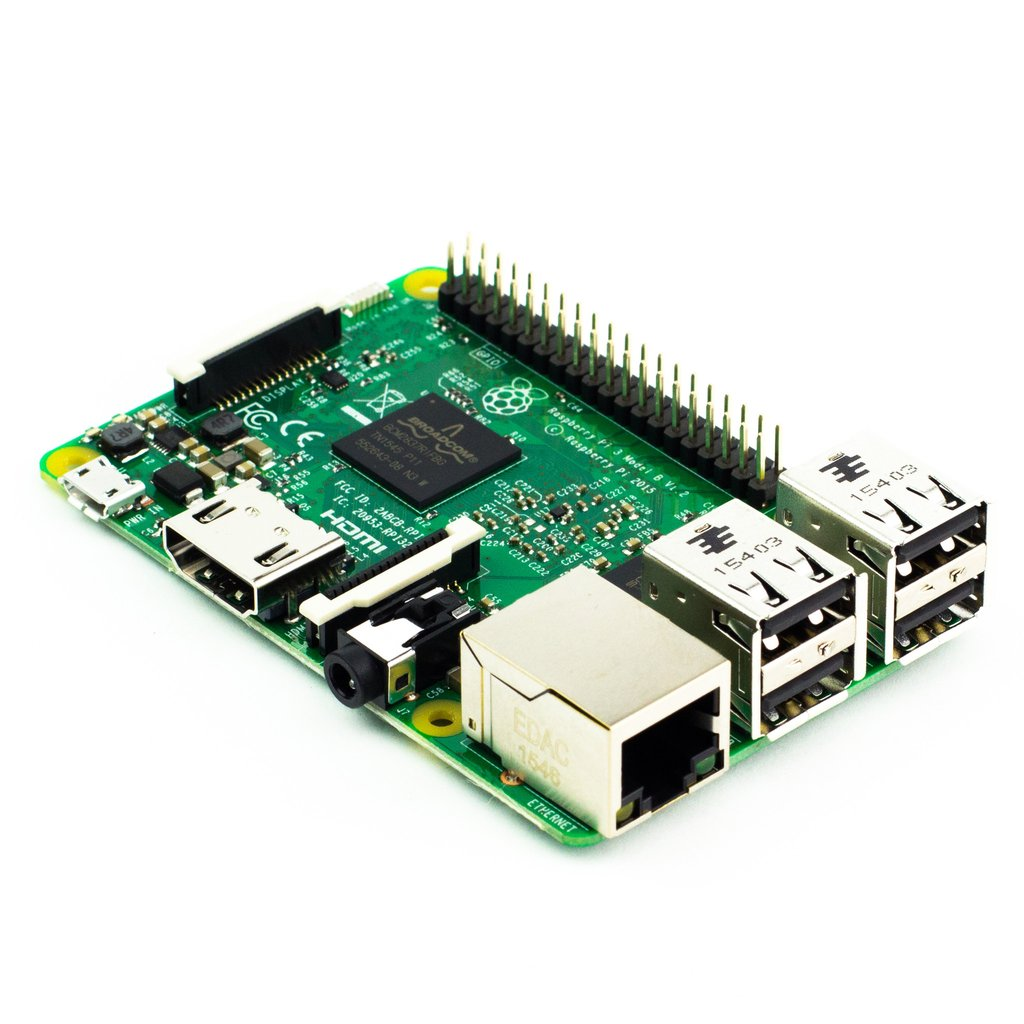
\includegraphics[width=3.5in, height=3in]{images/raspberry_pi.png}
	\caption{Raspberry Pi 3}
\end{figure}
\subsection{BeagleBone Black}
The BeagleBoard is a low-power open-source hardware single-board computer produced by Texas Instruments in association with Digi-Key and Newark element14. The BeagleBoard was also designed with open source software development in mind, and as a way of demonstrating the Texas Instrument's OMAP3530 system-on-a-chip. The board was developed by a small team of engineers as an educational board that could be used in colleges around the world to teach open source hardware and software capabilities. It is also sold to the public under the Creative Commons share-alike license. The board was designed using Cadence OrCAD for schematics and Cadence Allegro for PCB manufacturing; no simulation software was used.\\
The BeagleBone Black is the newest member of the BeagleBoard family. It is a lower-cost, high-expansion focused BeagleBoard using a low cost Sitara XAM3359AZCZ100 Cortex A8 ARM processor from Texas Instruments. It is similar to the Beaglebone,but with some features removed and some features added. The table below gives the high points on the differences between the BeagleBone and BeagleBone Black.
\begin{figure}[ht]
	\centering
	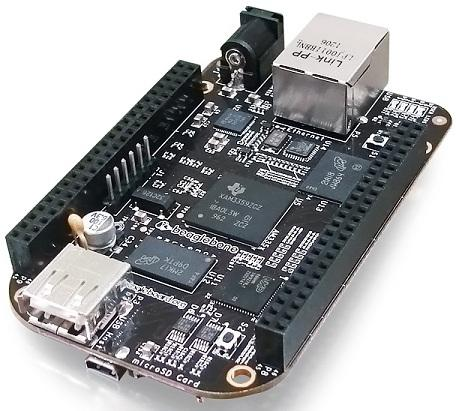
\includegraphics[width=3.5in, height=3in]{images/beaglebone_black.png}
	\caption{BeagleBone Black}
\end{figure}
\section{Tools used}
\subsection{Buildroot}
Buildroot is a set of Makefiles and patches that simplifies and automates the process of building a complete and bootable Linux environment for an embedded system, while using cross-compilation to allow building for multiple target platforms on a single Linux-based development system. Buildroot can automatically build the required cross-compilation toolchain, create a root file system, compile a Linux kernel image, and generate a boot loader for the targeted embedded system, or it can perform any independent combination of these steps. For example, an already installed cross-compilation toolchain can be used independently, while Buildroot only creates the root file system. \\
Buildroot is primarily intended to be used with small or embedded systems based on various computer architectures and instruction set architectures (ISAs), including x86, ARM, MIPS and PowerPC. Numerous architectures and their variants are supported; Buildroot also comes with default configurations for several off-the-shelf available embedded boards, such as Cubieboard, Raspberry Pi and SheevaPlug. Several third-party projects and products use Buildroot as the basis for their build systems, including the OpenWrt project that creates an embedded operating system, and firmware for the customer-premises equipment (CPE) used by the Google Fiber broadband service.\\
Multiple C standard libraries are supported as part of the toolchain, including the GNU C Library, uClibc and musl, as well as the C standard libraries that belong to various preconfigured development environments, such as those provided by Linaro. Buildroot's build configuration system internally uses Kconfig, which provides features such as a menu-driven interface, handling of dependencies, and contextual help; Kconfig is also used by the Linux kernel for its source-level configuration. Buildroot is organized around numerous automatically downloaded packages, which contain the source code of various userspace applications, system utilities, and libraries. Root file system images, which are the final results, may be built using various file systems, including cramfs, JFFS2, romfs, SquashFS and UBIFS.\\
Buildroot is free and open-source software, maintained by Peter Korsgaard and licensed under version 2 or later of the GNU General Public License (GPL). The project started in 2001, with initial intentions to serve as a testbed for uClibc. New releases are made available every three months.
\begin{figure}[ht]
	\centering
	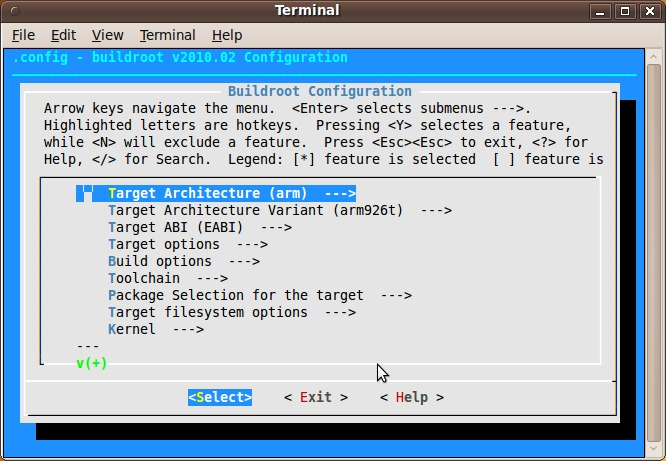
\includegraphics[width=3.5in, height=3in]{images/buildroot.png}
	\caption{Buildroot}
\end{figure}
\subsection{Cscope}
While hacking around the Linux source code it becomes very difficult to keep track of the program flow or the variable structures in your head. There isn’t any IDE to help out in source code browsing either. In such situation a tool is necessary that browses source code and is based on the terminal. This is where cscope comes into picture.\\
cscope is a programming tool which works in console mode, text-based interface, that allows computer programmers or software developers to search source code of the programming language C, with some support for C++ and Java. It is often used on very large projects to find source code, functions, declarations, definitions and regular expressions given a text string. cscope is free and released under a BSD license. The original developer of cscope is \textbf{Joe Steffen}.\\
The history of the tool goes back to the days of the PDP-11, but it is still used by developers who are accustomed to using the vi or Vim editor or other text-based editors, instead of editors based on graphical user interfaces (GUI)s. The functions in cscope are available to varying degrees in modern graphical source editors.
cscope is used in two phases. First a developer builds the cscope database. The developer can often use find or other Unix tools to get the list of filenames needed to index into a file called cscope.files. The developer then builds a database using the command cscope -b -q -k. The k flag is intended to build a database for an operating system or C library source code. It will not look in /usr/include. Second, the developer can now search those files using the command cscope -d. Often an index must be rebuilt whenever changes are made to files.\\
In software development it is often very useful to be able to find the callers of a function because this is the way to understand how code works and what other parts of the program expect from a function. cscope can find the callers and callees of functions, but it is not a compiler and it does that by searching the text for keywords. This has the disadvantages that macros and duplicate symbol names can generate an unclear graph. There are other programs that can extract this information by parsing the source code or looking at the generated object files.
cscope was created to search content within C files, but it can also be used (with some limits) for C++ and Java files.
\begin{figure}[ht]
	\centering
	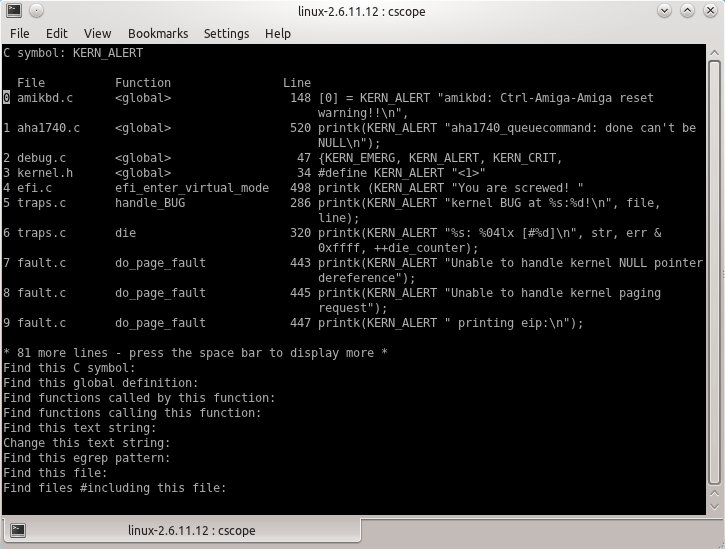
\includegraphics[scale=0.5]{images/cscope.png}
	\caption{Source Browsing through Cscope}
\end{figure}
\section{Testing}
The driver's job is to send commands from the Bluez stack to the device and get back its response. If all of this happens successfully then that should mean that the BlueNRG is able to communicate with another device using some BLE use cases.\\
Some of the use cases that can be used to test this are:
\begin{itemize}
	\item \textbf{Checking to see if BLE gets enabled}: 
		\begin{enumerate}
			\item This can be done using the following command\\
				\textbf{sudo hciconfig hci0 lestates}
			\item This command should return the following output:
				\begin{figure}[ht]
				\centering
				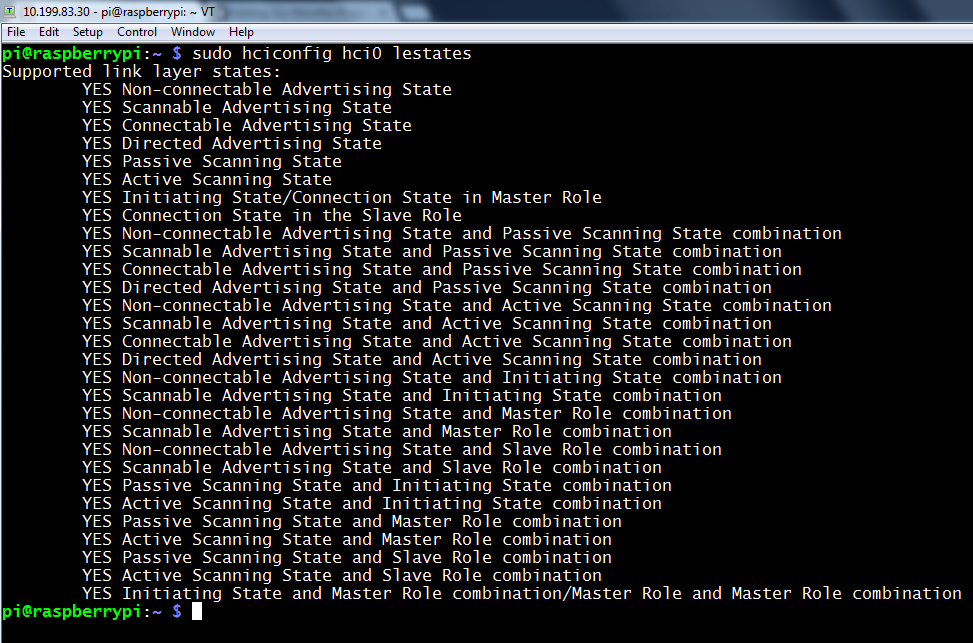
\includegraphics[scale=0.5]{images/lestates.png}
				\caption{List of LE states supported by adapter}
			\end{figure}
		\end{enumerate}
	\item \textbf{BLE gatttool interaction}: gatttool is one of the best methods to interact with another BLE device interactively from a Linux host. It opens an interactive session.
		\begin{enumerate}
			\item Find out the MAC\_ADDR of the other device using\\
				\textbf{sudo hcitool lescan}
				\begin{figure}[ht]
					\centering
					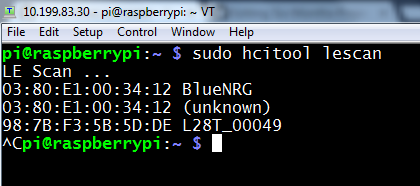
\includegraphics[scale=0.5]{images/lescan.png}
					\caption{List of LE devices scanned}
				\end{figure}
			\item Open interactive session using gatttool:\\
				\textbf{sudo gatttool -i hci0 -b MAC\_ADDR -I}
			\item In the interactive sesssion type in the following commands:\\
				\textbf{connect}
			\item Read profiles:\\
				\textbf{primary}
			\item Read all available characterstics:\\
				\textbf{char-desc}
				\begin{figure}[ht]
					\centering
					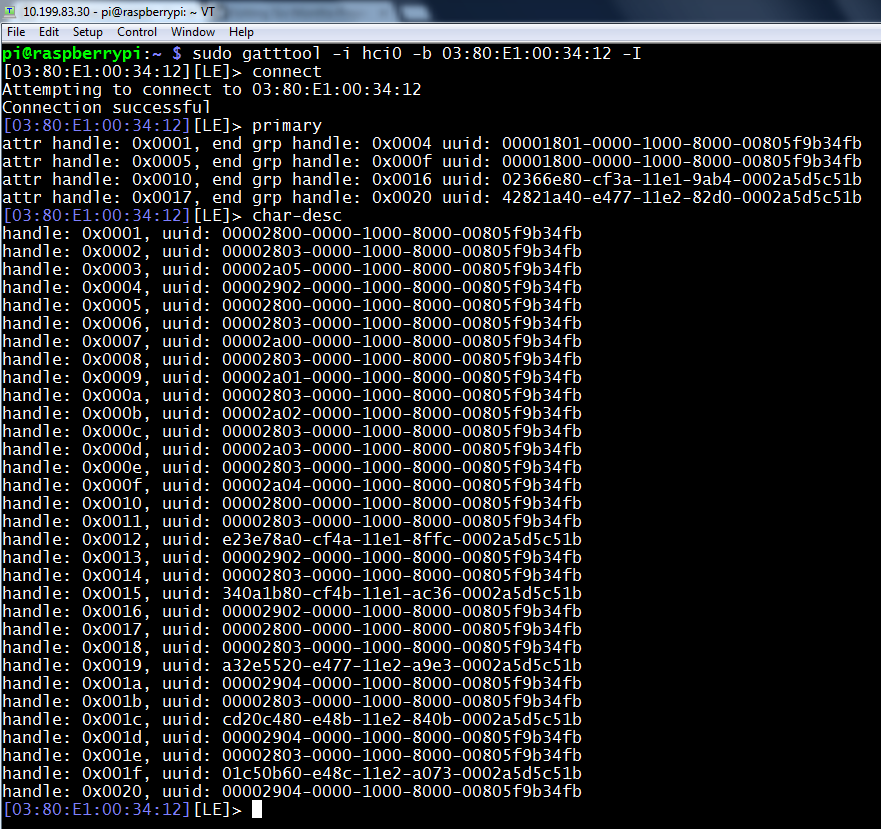
\includegraphics[scale=0.5]{images/gatttool1.png}
					\caption{GATTtool interaction part-I}
				\end{figure}
			\item Read the value of a characterstic:\\
        			\textbf{char-read-hnd The\_characterstic\_handle}
    			\item Write to a particular characterstc:\\
        			\textbf{char-write-cmd handle Value\_in\_Hex}
				\begin{figure}[ht]
					\centering
					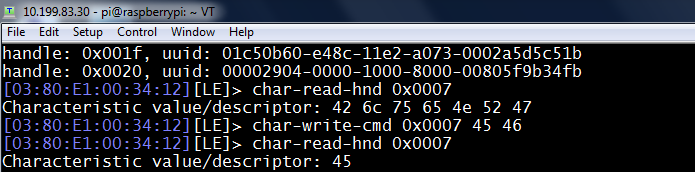
\includegraphics[scale=0.5]{images/gatttool2.png}
					\caption{GATTtool interaction part-II}
				\end{figure}
    			\item Disconnect:\\
        			\textbf{disconnect}
    			\item Quit:\\
        			\textbf{quit}
		\end{enumerate}
	\item \textbf{Reading Beacons using BLE}: 
		\begin{enumerate}
			\item There is a python script that can be used for this purpose, install it:\\
				\textbf{git clone https://github.com/switchdoclabs/BeaconAirPython.git}
			\item In order to use, the following package must be installed:
				\textbf{sudo apt-get install python-bluez}
			\item Scan and Read the beacons:\\
				\textbf{cd BeanconAirPython/ble}\\
				\textbf{sudo python testblescan.py}
			\item This should list out the nearby beacons:
				\begin{figure}[ht]
					\centering
					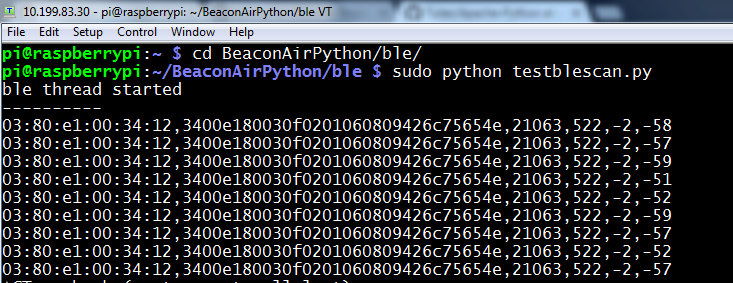
\includegraphics[scale=0.5]{images/beacon_read.png}
					\caption{Reading beacons}
				\end{figure}
		\end{enumerate}
	\item \textbf{Advertising with Beacons}:
		\begin{enumerate}
			\item Start advertising in non-connectable state:\\
				\textbf{sudo hciconfig hci0 leadv 3}\\
				\textbf{sudo hciconfig hci0 noscan}
			\item Broadcast a beacon:\\
				\textbf{HAHAHAH}
			\item You should see the following as output:
				\begin{figure}[ht]
					\centering
					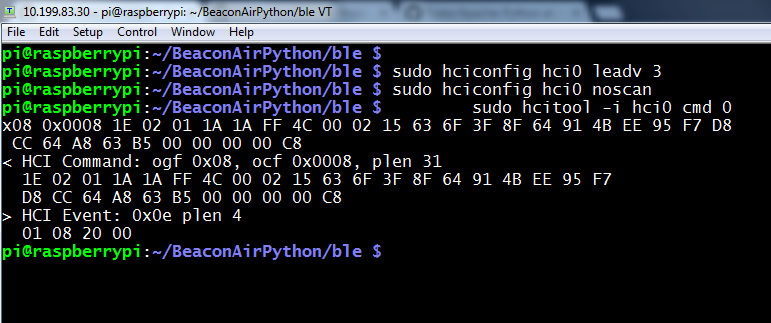
\includegraphics[scale=0.5]{images/advertising_beacons.png}
					\caption{Advertising using beacons}
				\end{figure}
		\end{enumerate}
\end{itemize}

